\section{Deep Neural Networks}

The perceptron, a simple neural-network model, fails on nonlinearly separable data because it can only draw a linear decision boundary.
\begin{figure}[ht]
    \centering
    \begin{minipage}{0.3\linewidth}
        \centering
        \begin{tabular}{|c|c||c|}
            \hline
            $x_1$ & $x_2$ & $x_1 \oplus x_2$ \\
            \hline
            0 & 0 & 0 \\
            0 & 1 & 1 \\
            1 & 0 & 1 \\
            1 & 1 & 0 \\
            \hline
        \end{tabular}
        \caption*{Truth table}
    \end{minipage}%
    \hfill
    \begin{minipage}{0.3\linewidth}
        \centering
        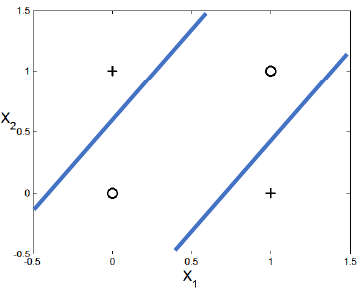
\includegraphics[width=0.6\linewidth]{img/xor_example.png}
        \caption*{Graphical representation}
    \end{minipage}%
    \hfill
    \begin{minipage}{0.3\linewidth}
        \centering
        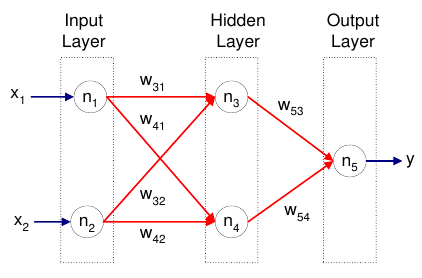
\includegraphics[width=0.7\linewidth]{img/XOR_NN.png}
        \caption*{Neural network diagram}
    \end{minipage}

    \caption{XOR: truth table, graphical representation, and neural network implementation}
    \label{fig:xor-combined}
\end{figure}


\begin{definition}[Deep learning]
\textbf{Deep learning} refers to representation-learning methods that let a machine take in raw data and automatically discover the representations needed for detection or classification.
\end{definition}

\begin{wrapfigure}{r}{0.3\linewidth}
    \centering
    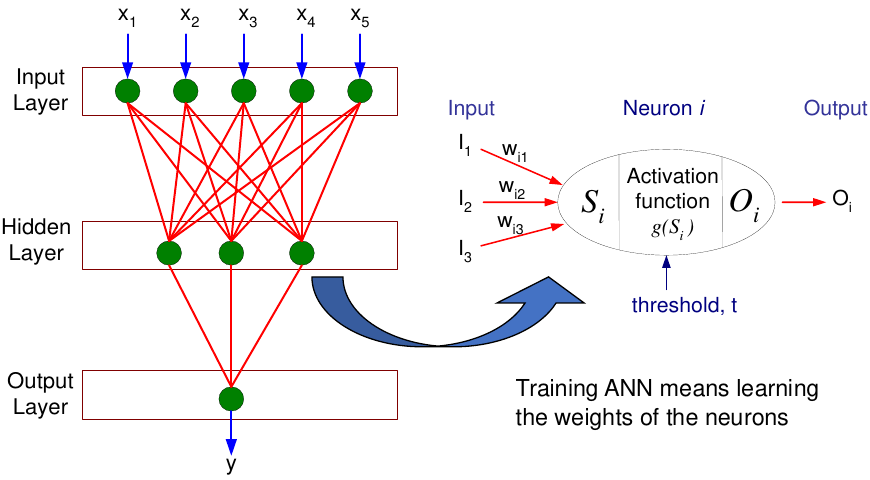
\includegraphics[width=\linewidth]{img/General_NN.png}
    \caption{NN structure}
    \label{fig:NN-structure}
\end{wrapfigure}


Deep learning systems transform raw input data into increasingly abstract representations. A multilayer neural network contains:
\begin{itemize}
    \item \textbf{input layer} (\textit{receives the initial data});
    \item \textbf{hidden layers} (\textit{intermediate layers between input and output});
    \item \textbf{output layer} (\textit{produces the final result}).
\end{itemize}


Unlike the single-layer perceptron, multilayer networks solve nonlinear classification tasks. We can read each hidden node as a perceptron that builds one hyperplane, and the output node combines these hyperplanes into a complex decision boundary. Training an artificial neural network (ANN) means learning the weight values that make these boundaries fit the data.

\begin{equation}
\overbrace{O_i}^{\text{output}}  = \overbrace{g\left(\underbrace{\sum_j \overbrace{I_j}^{\text{input}} \cdot \overbrace{w_{ij}}^{\text{weight}}}_{\text{weighted sum } S_i}\right)}^\text{activation function}\qquad\text{neuron function}\label{neuron-func}
\end{equation}

Deep neural networks contain multiple hidden layers, and each added layer lets the network learn a more abstract representation of the data. Rather than fixing by hand the right levels of abstraction for processing information, deep learning lets the model discover these representations on its own.

\subsection{Activation Functions}
Activation functions introduce nonlinearity into a neural network, which is what lets it learn complex patterns.
\begin{figure}[ht]
\centering

\begin{minipage}{0.3\textwidth}
    \centering
    \textbf{Tanh}
\end{minipage}
\hfill
\begin{minipage}{0.3\textwidth}
    \centering
    \textbf{ReLU}
\end{minipage}
\hfill
\begin{minipage}{0.3\textwidth}
    \centering
    \textbf{Soft Exponential}
\end{minipage}

\vspace{1em}

\begin{minipage}{0.3\textwidth}
    \centering
    $f(x) = \tanh(x) = \dfrac{e^x - e^{-x}}{e^x + e^{-x}}$
\end{minipage}
\hfill
\begin{minipage}{0.3\textwidth}
    \centering
    $f(x) =
    \begin{cases}
        0 & x < 0 \\
        x & x \geq 0
    \end{cases}$
\end{minipage}
\hfill
\begin{minipage}{0.3\textwidth}
    \centering
    $f(x) = \log(e^x + 1)$
\end{minipage}

\vspace{1em}

\begin{minipage}{0.3\textwidth}
    \centering
    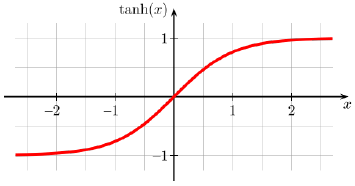
\includegraphics[width=0.8\linewidth]{img/tanh.png}
\end{minipage}
\hfill
\begin{minipage}{0.3\textwidth}
    \centering
    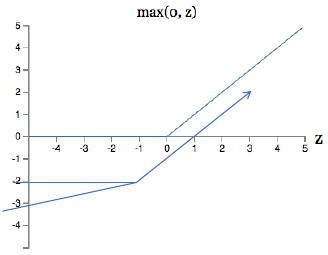
\includegraphics[width=0.8\linewidth]{img/ReLU.png}
\end{minipage}
\hfill
\begin{minipage}{0.3\textwidth}
    \centering
    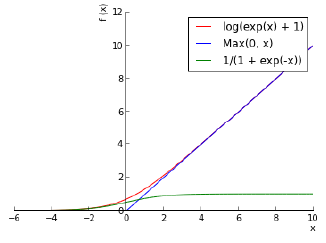
\includegraphics[width=0.8\linewidth]{img/soft-exponential-linear.png}
\end{minipage}

\vspace{1em}

\begin{minipage}{0.3\textwidth}
    \centering
    \small
    Similar to sigmoid but ranges from $-1$ to $+1$. Zero-centered; better for gradients than sigmoid.
\end{minipage}
\hfill
\begin{minipage}{0.3\textwidth}
    \centering
    \small
    Efficient and widely used. May cause ``dying ReLU'' for $x < 0$ due to zero gradient.
\end{minipage}
\hfill
\begin{minipage}{0.3\textwidth}
    \centering
    \small
    Smooth version of ReLU. Doesn't saturate, promotes sparsity, mitigates vanishing gradient.
\end{minipage}

\caption{Activation functions: formula, graph, and properties}
\end{figure}


\begin{figure}[h]
    \centering
    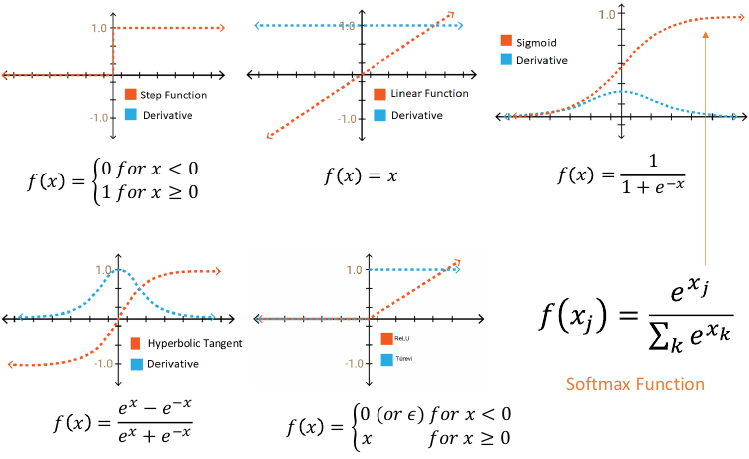
\includegraphics[width=0.5\linewidth]{img/ActivationFunctionSummary.png}
    \caption{most common activation functions}
    \label{fig:07-lbl1}
\end{figure}

\subsection{Training Neural Networks}
The hard part of training a multilayer network is finding the true error of the hidden nodes. At the output nodes the error is easy: it is the difference between predicted and actual values. Hidden nodes have no direct target, so their share of the error is not given.

\subsubsection{Gradient Descent for Multilayer Neural Networks}

Gradient descent (GD) is an optimization algorithm for training neural networks. It minimizes the error function (\ref{error function}) through the weight update (\ref{weights update}).
\begin{align}
\overbrace{E}^{\text{error to minimize}} &= \frac{1}{2} \sum_{i=1}^{N}  \overbrace{\left(t_i - f(w_j \cdot x_{ij})\right)^2}^{\text{sum of squared residuals}} \label{error function}
\\
\overbrace{w_j^{(k+1)}}^{\text{weight at iteration $k+1$}} &= w_j^{(k)} - \underbrace{\eta}_{\text{learning rate}} \times\overbrace{\frac{\partial E}{\partial w_j}}^{\text{activation function's slope}}\label{weights update}
\end{align}

\begin{example}[sigmoid function]
\begin{equation}
w_j^{(k+1)} = w_j^{(k)} + \eta\sum_i (t_i - o_i) \cdot o_i \cdot (1 - o_i) \cdot x_{ij}
\end{equation}
\end{example}
For output neurons, the weight-update formula is the same as before (\textit{GD for perceptron}). For hidden neurons, it becomes (\ref{weightHidden}).
\begin{align}
w_{pi}^{(k+1)} & = w_{pi}^{(k)} + \eta \cdot o_i \cdot (1 - o_i) \cdot x_p \cdot \sum_j \delta_j \cdot w_{ij}\label{weightHidden}
\\
\delta_j & = o_j(1-o_j)(t_j-o_j) & \text{output neurons}
\\
\delta_j & = o_j(1-o_j)\sum_{k \in \phi_j}\delta_k w_{jk} & \text{hidden neurons}
\end{align}
\newpage
\begin{figure}[h]
\centering
\begin{minipage}{0.27\textwidth}
    \begin{adjustbox}{max width=\textwidth}
    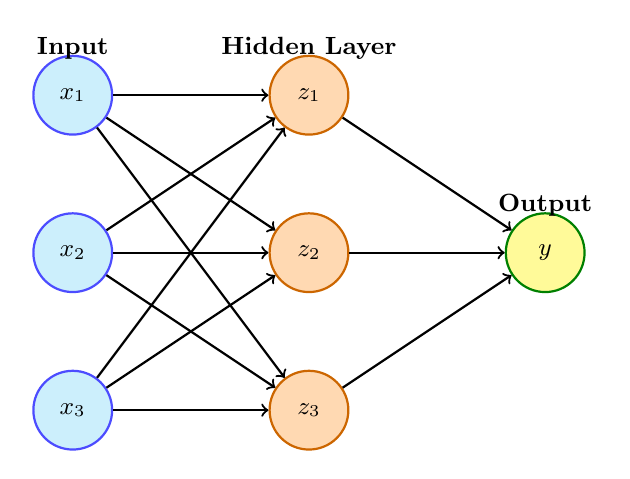
\begin{tikzpicture}[node distance=0.5cm and 0.5cm, every node/.style={font=\small}]
    
    \node[circle, draw=blue!70, fill=cyan!20, thick, minimum size=1cm] (x1) at (0, 2) {$x_1$};
    \node[circle, draw=blue!70, fill=cyan!20, thick, minimum size=1cm] (x2) at (0, 0) {$x_2$};
    \node[circle, draw=blue!70, fill=cyan!20, thick, minimum size=1cm] (x3) at (0, -2) {$x_3$};
    
    \node[circle, draw=orange!80!black, fill=orange!30, thick, minimum size=1cm] (z1) at (3, 2) {$z_1$};
    \node[circle, draw=orange!80!black, fill=orange!30, thick, minimum size=1cm] (z2) at (3, 0) {$z_2$};
    \node[circle, draw=orange!80!black, fill=orange!30, thick, minimum size=1cm] (z3) at (3, -2) {$z_3$};
    
    \node[circle, draw=green!50!black, fill=yellow!40, thick, minimum size=1cm] (y) at (6, 0) {$y$};
    
    \foreach \i in {1,2,3} {
      \foreach \j in {1,2,3} {
        \draw[->, thick] (x\i) -- (z\j);
      }
    }
    
    \foreach \j in {1,2,3} {
      \draw[->, thick] (z\j) -- (y);
    }
    
    \node at (0, 2.6) {\textbf{Input}};
    \node at (3, 2.6) {\textbf{Hidden Layer}};
    \node at (6, 0.6) {\textbf{Output}};
    \end{tikzpicture}
    \end{adjustbox}

    \vspace{0.5cm}

    \begin{adjustbox}{max width=\textwidth}
    \begin{tikzpicture}[node distance=0.5cm and 0.5cm, every node/.style={font=\small}]
    
    \node[draw, thick, rounded corners, minimum width=5.2cm, align=center] (loss) {\textbf{(F) Loss} \\
    $E = \frac{1}{2}(y - y^*)^2$};
    
    \node[draw, thick, rounded corners, minimum width=5.2cm, align=center, below=of loss] (out_sigmoid) {\textbf{(E) Output (sigmoid)} \\
    $y = \frac{1}{1 + \exp(-b)}$};
    
    \node[draw, thick, rounded corners, minimum width=5.2cm, align=center, below=of out_sigmoid] (out_linear) {\textbf{(D) Output (linear)} \\
    $b = \sum_{j=0}^D \beta_j z_j$};
    
    \node[draw, thick, rounded corners, minimum width=5.2cm, align=center, below=of out_linear] (hid_sigmoid) {\textbf{(C) Hidden (sigmoid)} \\
    $z_j = \frac{1}{1 + \exp(-a_j)}$};
    
    \node[draw, thick, rounded corners, minimum width=5.2cm, align=center, below=of hid_sigmoid] (hid_linear) {\textbf{(B) Hidden (linear)} \\
    $a_j = \sum_{i=0}^M \alpha_{ji} x_i$};
    
    \node[draw, thick, rounded corners, minimum width=5.2cm, align=center, below=of hid_linear] (input) {\textbf{(A) Input} \\
    Given $x_i$, $\forall i$};
    
    \foreach \i/\j in {loss/out_sigmoid, out_sigmoid/out_linear, out_linear/hid_sigmoid, hid_sigmoid/hid_linear, hid_linear/input} {
      \draw[<-, thick] (\i.south) -- (\j.north);
    }
    \end{tikzpicture}
    \end{adjustbox}
\end{minipage}
\hfill
\begin{minipage}{0.7\textwidth}
    \textbf{\textit{Forward propagation} in a NN consisting of one hidden layer.}
    
    The network has the \textbf{input layer} (\textit{blue}), the \textbf{hidden layer} (\textit{orange}), and the \textbf{output layer} (\textit{yellow}). 
    
    Each neuron in one layer connects to all neurons in the next layer through weighted edges. Here $\alpha_{ji}$ denotes the weights on connections from the input layer to the hidden layer, and $\beta_j$ those from the hidden layer to the output layer.

    The top diagram shows this architecture; the bottom one lays out the mathematical operations of the forward pass, step by step.

    \begin{enumerate}
    \item[A] \textit{[input]} $x_i$.
    \item[B] \textit{[hidden layer]} each $x_i$ is linearly combined with the weights $\alpha_{ji}$ to compute the activation $a_j$ for each hidden neuron.
    \item[C] \textit{[hidden layer]} each $a_j$ is passed through an activation function (typically the sigmoid function) to compute the output $z_j$
    \item[D] \textit{[output layer]} $z_j$, are combined with the weights $\beta_j$ to compute the final linear sum $b$;
    \item[E] \textit{[output layer]} $b$ is passed through another activation function (again, typically a sigmoid) to produce the final output $y$
    \item[F] \textit{[loss]} the final output $y$ is compared with the expected output $y^*$ through a loss function $E$. A common choice is the mean squared error (MSE) or cross-entropy loss, depending on the task. At this stage the loss $E$ is known only at the output layer.
    \end{enumerate}
    \textbf{How do we update these weights, including those in the hidden layer, when the loss is available only at the output?}
    The \textbf{backpropagation algorithm} solves this: it propagates the error backward through the network to compute gradients and update every weight. We compute the gradient of the loss with respect to each weight, then step each weight in the direction that lowers the loss.
\end{minipage}
\end{figure}


\subsubsection{Error Backpropagation}
Backpropagation tunes the weights of a neural network so that it maps inputs to the correct outputs.

\begin{enumerate}
    \item \textbf{Forward Pass} Compute the network output
    \begin{itemize}
        \item Compute net inputs: Weighted sum of inputs for each neuron.
        \item Apply activation function: Typically a sigmoid function.
        \item Propagate values: Pass values to the next layer.
        \item Calculate final output: Based on values from previous layers.
    \end{itemize}

    \item \textbf{Calculate Error} The total error is the sum of squared differences between actual and desired outputs.

    \item \textbf{Backward Pass}  Compute the loss function gradients and update weights
    \begin{itemize}
        \item Compute gradients: Use the chain rule to determine weight effects on error.
        \item Propagate error: Backward through the network to update weights.
        \item Derive delta rule: Calculate weight updates based on error gradients.
        \item Apply learning rate: Update weights in the opposite direction of the gradient.
    \end{itemize}
\end{enumerate}

\textbf{Goal:} minimize the total error by adjusting the weights, so the network produces the correct output for each input.

\paragraph{Key Importance of Error Functions}
The error (loss, cost) function reduces every aspect of the system to a single scalar, so that candidate solutions can be compared. A poor choice of error function leads to poor results: specifying the goal correctly is therefore half the work.

\subsubsection{Objective Functions}
\textbf{Regression:} the output layer is a single node with a linear activation function, which lets the network predict any value in a continuous range. The standard loss for regression is the quadratic loss, also known as mean squared error (MSE), which penalizes the squared difference between prediction and target:
\begin{equation}
    J = \frac{1}{2}(y - y^*)^2
\end{equation}
During backpropagation, the gradient is calculated as:
\begin{equation}
\frac{dJ}{dy} = y - y^*    
\end{equation}

\textbf{Classification:} the architecture depends on the number of classes. For \textit{binary classification} ($K=2$), a single node with a sigmoid activation suffices, and its output is the probability of the positive class. For \textit{multi-class problems} ($K>2$), the output layer uses $K$ nodes with a softmax to produce a probability distribution over the classes; here the target variable must be one-hot encoded.

The standard loss for classification is the cross-entropy, equivalent to the negative log-likelihood:
\begin{equation}
J = -\sum y^* \log(y)
\end{equation}
For binary classification specifically, the cross-entropy formula is:
\begin{equation}
J = -\left(y^* \log(y) + (1 - y^*)\log(1 - y)\right)    
\end{equation}
The gradient during backpropagation for binary classification is:
\begin{equation}
\frac{dJ}{dy} = -y^* \frac{1}{y} - (1 - y^*)\frac{1}{y - 1}
\end{equation}
In these equations $y$ is the predicted value or probability, while $y^*$ is the actual target value or label.
\paragraph{Design Issues in ANN}
The main choices when designing a neural network are:

\begin{itemize}
\item Input layer size:
  \begin{itemize}
  \item One node per binary/continuous attribute
  \item $k$ or $\log_2 k$ nodes for categorical attributes with $k$ values
  \end{itemize}
  
\item Output layer size:
  \begin{itemize}
  \item One node for binary classification
  \item $k$ or $\log_2 k$ nodes for $k$-class problems
  \end{itemize}
  
\item Hidden layer size and number
\item Initial weights and biases
\end{itemize}

\paragraph{Characteristics of ANN}
Neural networks share several traits worth keeping in mind:

\begin{itemize}
\item Multilayer ANNs are universal approximators, but may overfit if too large
\item Gradient descent can converge to a local minimum
\item Model building is often slow, while inference is fast
\item They handle redundant attributes well, since the weights are learned automatically
\item They are sensitive to noise in the training data
\item They struggle with missing attributes
\end{itemize}
\subsection{Tips and Tricks for Neural Network Training}

\paragraph{Dataset Splitting}
Split the dataset three ways. The \textbf{training set} updates the weights, its records processed repeatedly in random order. The \textbf{validation set} tells us when to stop training, by monitoring the error, and lets us pick the best model configuration. The \textbf{test set} measures the final performance of the network and must stay untouched during development.

\paragraph{Weight Initialization} The initial weights matter because they fix the starting position in weight space. Draw them randomly from a uniform distribution, normalized so that the number of weighted connections per unit yields midrange signals. Trying several random initializations tests how stable the result is and improves the odds of reaching a good optimum.

\paragraph{Learning Modes} There are three main learning modes:

\begin{itemize}
\item Sequential mode (online/stochastic/per-record):
  \begin{itemize}
  \item Weights updated after each record
  \item Many weight updates can lead to quicker convergence but less stable learning
  \end{itemize}
  
\item Batch mode (offline/per-epoch):
  \begin{itemize}
  \item Weights updated after all records are processed
  \item Can be slow and may get trapped in early local minima
  \end{itemize}
  
\item Minibatch mode (a blend of the above):
  \begin{itemize}
  \item Weights updated after processing a subset of records (tens to thousands)
  \item Combines benefits of both approaches
  \item Well-suited for GPU acceleration
  \end{itemize}
\end{itemize}

\paragraph{Convergence Criteria} Training needs a stopping criterion to define convergence. The Euclidean norm of the gradient vector should reach a sufficiently small value, and the absolute rate of change of the average squared error per epoch should become sufficiently small. To watch generalization, we stop when performance on held-out data peaks.

\paragraph{Early Stopping} Running too many epochs invites overfitting. Keep a hold-out validation set, test accuracy after every epoch, save the weights of the best network on that set, and stop once the error climbs past this point. Let the network run a few epochs before deciding to stop (the patience parameter). The training error keeps falling, while the validation error eventually turns upward: that turn signals overfitting.

\paragraph{Model Selection}
Finding the right network size matters. Too few hidden units and the network cannot learn enough; too many and it overfits, unless properly regularized. Cross-validation fixes the number of hidden units, using the validation error to select the best architecture.

\paragraph{Regularization}

Regularization constrains the learning model to avoid overfitting and improve generalization:

\begin{equation}
E' = E(y, y^*) + \lambda R(\cdot)
\end{equation}

where $E(y, y^*)$ is the original error function, $\lambda$ is a hyperparameter chosen during model selection, and $R(\cdot)$ is a penalty term that can be applied to parameters ($R(W_\theta)$) or activations ($R(Z)$).

\paragraph{Common Penalty Terms}

Common regularization norms include the 1-norm: $||A||_1 = \sum_{ij} |a_{ij}|$, which can be applied to parameters ($R(W_\theta) = ||W_\theta||_1$) or activations ($R(Z(X)) = ||Z(X)||_1$); and the 2-norm: $||A||_2 = \sqrt{\sum_{ij} a_{ij}^2}$, which can be applied to parameters ($R(W_\theta) = ||W_\theta||_2^2$) or activations ($R(Z(X)) = ||Z(X)||_2^2$).

\paragraph{Dropout Regularization} Dropout randomly disconnects units from the network during training. A unit-dropping hyperparameter controls it. It prevents units from co-adapting, produces a committee-machine effect, needs an adjustment at prediction time, and can return predictions with confidence intervals. Applied to individual connections instead of units, it becomes dropconnect.

\paragraph{Momentum} Adding a momentum term to the weight-update equation stores an exponentially weighted history of past weight changes; this damps instability and speeds up convergence. When successive weight changes share the same sign, momentum grows and accelerates convergence over shallow gradients. When they have opposite signs, momentum shrinks and oscillations die down. The stored history can also help the network escape a local minimum.

\paragraph{Choosing the Optimization Algorithm} Several optimization algorithms are available:

\begin{itemize}
\item Standard stochastic gradient descent (SGD): easy and efficient, but the optimal learning rate is hard to pick and convergence is unstable; often paired with momentum.

\item RMSprop: an adaptive learning-rate method that scales the rate down using a moving average of squared gradients, speeding up convergence where gradients are steep.

\item Adagrad: similar to RMSprop, but with element-wise gradient scaling.

\item ADAM: combines Adagrad with an exponentially decaying average of past gradients (like momentum).
\end{itemize}
\subsection{Advanced Neural Network Architectures}

\subsubsection{Convolutional Neural Networks (CNN)}

\textbf{CNNs} are specialized architectures, applied mostly to classifying images and time-series data. In a fully connected layer each neuron connects to every neuron of the previous layer; a convolutional layer instead uses filters (kernels) that slide across the input:

\begin{itemize}
\item Filters always extend to the full depth of the input volume
\item Each filter produces an activation map by computing dot products at each position
\item Convolution kernels detect specific features (e.g., edges, textures)
\end{itemize}

\begin{figure}[h]
    \centering
    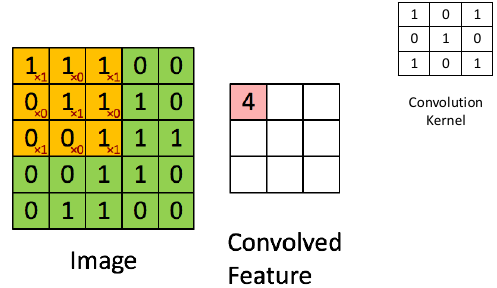
\includegraphics[width=0.5\linewidth]{img/example of convolution layer.png}
    \caption{example of convolution layer}
    \label{conv-layer}
\end{figure}
\paragraph{CNN Architecture}

A CNN is a stack of convolutional layers, each followed by an activation function. The layers progressively shrink the spatial dimensions of the input volumes, so the network extracts steadily more abstract features. Shrink them too fast, though, and performance drops: too little spatial information survives. The rate of reduction therefore needs care, keeping the important features while still cutting the dimensions down.

\paragraph{CNN Components}
The key CNN concepts are:

\begin{itemize}
\item Stride: the step size with which the filter moves across the input (i.e. how many pixels we ``jump'' after each computation)
\item Padding: adding border pixels to the input to control the output dimensions
\item Pooling layers: operations that reduce the spatial dimensions
  \begin{itemize}
  \item MaxPooling: Takes the maximum value in a region
  \item AvgPooling: Computes the average value in a region
  \end{itemize}
\end{itemize}

\paragraph{Convolution Summary}    
Accepts a volume of size $W_1 \times H_1 \times D_1$. Requires four hyperparameters:
    \begin{itemize}
        \item Number of filters $K$,
        \item their spatial extent $F$,
        \item the stride $S$,
        \item the amount of zero padding $P$.
    \end{itemize}
Produces a volume of size $W_2 \times H_2 \times D_2$ where:
    \begin{itemize}
        \item $W_2 = \frac{(W_1 - F + 2P)}{S} + 1$
        \item $H_2 = \frac{(H_1 - F + 2P)}{S} + 1$ (i.e. width and height are computed equally by symmetry)
        \item $D_2 = K$
    \end{itemize}
With parameter sharing, it introduces $F \cdot F \cdot D_1$ weights per filter, for a total of $(F \cdot F \cdot D_1) \cdot K$ weights and $K$ biases. In the output volume, the $d$-th depth slice (of size $W_2 \times H_2$) is the result of performing a valid convolution of the $d$-th filter over the input volume with a stride of $S$, and then offset by $d$-th bias.

\paragraph{Pooling Summary}
Accepts a volume of size $W_1 \times H_1 \times D_1$. Requires two hyperparameters: their spatial extent $F$ and the stride $S$. Produces a volume of size $W_2 \times H_2 \times D_2$ where:
    \begin{itemize}
        \item $W_2 = \frac{(W_1 - F)}{S} + 1$
        \item $H_2 = \frac{(H_1 - F)}{S} + 1$
        \item $D_2 = D_1$
    \end{itemize}
Introduces zero parameters since it computes a fixed function of the input. Note that it is not common to use zero-padding for Pooling layers.

\subsubsection{Recurrent Neural Networks (RNN)}

Recurrent Neural Networks (RNNs) process sequential data by keeping an internal state, a form of memory. This \textit{internal state} is updated as the network reads through the sequence.

\begin{equation}
    \overbrace{h_t}^{\text{state $t$}} = \underbrace{f_W(h_{t-1}, \overbrace{x_t}^{\text{input vector at timestep $t$}})}_{\text{function with parameter $W$}}
\end{equation}
\begin{figure}[h]
    \centering
    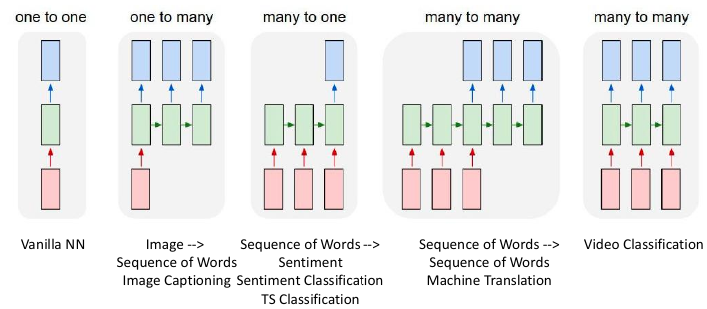
\includegraphics[width=0.5\linewidth]{img/RNNtypes.png}
    \caption{types of Recurrent Neural Network}
    \label{fig:07-lbl2}
\end{figure}

RNNs can be configured for various tasks:
\begin{itemize}
\item One-to-One: Standard neural network (image classification)
\item One-to-Many: Image to sequence of words (image captioning)
\item Many-to-One: Sequence to classification (sentiment analysis, time series classification)
\item Many-to-Many: Sequence to sequence (machine translation, video classification)
\end{itemize}

An RNN processes a sequence of vectors by applying a recurrence formula at each time step:

\begin{equation}
h_t = f(W_{hh} \cdot h_{t-1} + W_{xh} \cdot x_t)
\end{equation}
\begin{equation}
y_t = W_{hy} \cdot h_t
\end{equation}

The same weight matrices are reused at every time step, which lets the network handle sequences of variable length.

An RNN can be unfolded in time into a computational graph:
\begin{itemize}
\item Many-to-Many: output at each time step
\item Many-to-One: output only at the final time step
\end{itemize}
\textit{Note:} training propagates information forward and then backward through time. At test time the learned weights are applied to new sequences. In this way an RNN captures temporal dependencies in the data.

